\documentclass[twoside]{book}

% Packages required by doxygen
\usepackage{calc}
\usepackage{doxygen}
\usepackage{graphicx}
\usepackage[utf8]{inputenc}
\usepackage{makeidx}
\usepackage{multicol}
\usepackage{multirow}
\usepackage{textcomp}
\usepackage[table]{xcolor}

% Font selection
\usepackage[T1]{fontenc}
\usepackage{mathptmx}
\usepackage[scaled=.90]{helvet}
\usepackage{courier}
\usepackage{amssymb}
\usepackage{sectsty}
\renewcommand{\familydefault}{\sfdefault}
\allsectionsfont{%
  \fontseries{bc}\selectfont%
  \color{darkgray}%
}
\renewcommand{\DoxyLabelFont}{%
  \fontseries{bc}\selectfont%
  \color{darkgray}%
}

% Page & text layout
\usepackage{geometry}
\geometry{%
  a4paper,%
  top=2.5cm,%
  bottom=2.5cm,%
  left=2.5cm,%
  right=2.5cm%
}
\tolerance=750
\hfuzz=15pt
\hbadness=750
\setlength{\emergencystretch}{15pt}
\setlength{\parindent}{0cm}
\setlength{\parskip}{0.2cm}
\makeatletter
\renewcommand{\paragraph}{%
  \@startsection{paragraph}{4}{0ex}{-1.0ex}{1.0ex}{%
    \normalfont\normalsize\bfseries\SS@parafont%
  }%
}
\renewcommand{\subparagraph}{%
  \@startsection{subparagraph}{5}{0ex}{-1.0ex}{1.0ex}{%
    \normalfont\normalsize\bfseries\SS@subparafont%
  }%
}
\makeatother

% Headers & footers
\usepackage{fancyhdr}
\pagestyle{fancyplain}
\fancyhead[LE]{\fancyplain{}{\bfseries\thepage}}
\fancyhead[CE]{\fancyplain{}{}}
\fancyhead[RE]{\fancyplain{}{\bfseries\leftmark}}
\fancyhead[LO]{\fancyplain{}{\bfseries\rightmark}}
\fancyhead[CO]{\fancyplain{}{}}
\fancyhead[RO]{\fancyplain{}{\bfseries\thepage}}
\fancyfoot[LE]{\fancyplain{}{}}
\fancyfoot[CE]{\fancyplain{}{}}
\fancyfoot[RE]{\fancyplain{}{\bfseries\scriptsize Generated on Wed Nov 27 2013 00\-:19\-:41 for Documentacion by Doxygen }}
\fancyfoot[LO]{\fancyplain{}{\bfseries\scriptsize Generated on Wed Nov 27 2013 00\-:19\-:41 for Documentacion by Doxygen }}
\fancyfoot[CO]{\fancyplain{}{}}
\fancyfoot[RO]{\fancyplain{}{}}
\renewcommand{\footrulewidth}{0.4pt}
\renewcommand{\chaptermark}[1]{%
  \markboth{#1}{}%
}
\renewcommand{\sectionmark}[1]{%
  \markright{\thesection\ #1}%
}

% Indices & bibliography
\usepackage{natbib}
\usepackage[titles]{tocloft}
\setcounter{tocdepth}{3}
\setcounter{secnumdepth}{5}
\makeindex

% Hyperlinks (required, but should be loaded last)
\usepackage{ifpdf}
\ifpdf
  \usepackage[pdftex,pagebackref=true]{hyperref}
\else
  \usepackage[ps2pdf,pagebackref=true]{hyperref}
\fi
\hypersetup{%
  colorlinks=true,%
  linkcolor=blue,%
  citecolor=blue,%
  unicode%
}

% Custom commands
\newcommand{\clearemptydoublepage}{%
  \newpage{\pagestyle{empty}\cleardoublepage}%
}


%===== C O N T E N T S =====

\begin{document}

% Titlepage & ToC
\hypersetup{pageanchor=false}
\pagenumbering{roman}
\begin{titlepage}
\vspace*{7cm}
\begin{center}%
{\Large Documentacion \\[1ex]\large 1.\-0.\-0 }\\
\vspace*{1cm}
{\large Generated by Doxygen 1.8.5}\\
\vspace*{0.5cm}
{\small Wed Nov 27 2013 00:19:41}\\
\end{center}
\end{titlepage}
\clearemptydoublepage
\tableofcontents
\clearemptydoublepage
\pagenumbering{arabic}
\hypersetup{pageanchor=true}

%--- Begin generated contents ---
\chapter{Namespace Index}
\section{Packages}
Here are the packages with brief descriptions (if available)\-:\begin{DoxyCompactList}
\item\contentsline{section}{\hyperlink{namespacees}{es} }{\pageref{namespacees}}{}
\item\contentsline{section}{\hyperlink{namespacees_1_1ull}{es.\-ull} }{\pageref{namespacees_1_1ull}}{}
\item\contentsline{section}{\hyperlink{namespacees_1_1ull_1_1etsii}{es.\-ull.\-etsii} }{\pageref{namespacees_1_1ull_1_1etsii}}{}
\item\contentsline{section}{\hyperlink{namespacees_1_1ull_1_1etsii_1_1contexto}{es.\-ull.\-etsii.\-contexto} }{\pageref{namespacees_1_1ull_1_1etsii_1_1contexto}}{}
\item\contentsline{section}{\hyperlink{namespacees_1_1ull_1_1etsii_1_1estrategias}{es.\-ull.\-etsii.\-estrategias} }{\pageref{namespacees_1_1ull_1_1etsii_1_1estrategias}}{}
\item\contentsline{section}{\hyperlink{namespacees_1_1ull_1_1etsii_1_1main}{es.\-ull.\-etsii.\-main} }{\pageref{namespacees_1_1ull_1_1etsii_1_1main}}{}
\item\contentsline{section}{\hyperlink{namespacees_1_1ull_1_1etsii_1_1singleton}{es.\-ull.\-etsii.\-singleton} }{\pageref{namespacees_1_1ull_1_1etsii_1_1singleton}}{}
\end{DoxyCompactList}

\chapter{Hierarchical Index}
\section{Class Hierarchy}
This inheritance list is sorted roughly, but not completely, alphabetically\-:\begin{DoxyCompactList}
\item \contentsline{section}{es.\-ull.\-etsii.\-estrategias.\-I\-Behaviour}{\pageref{interfacees_1_1ull_1_1etsii_1_1estrategias_1_1_i_behaviour}}{}
\begin{DoxyCompactList}
\item \contentsline{section}{es.\-ull.\-etsii.\-estrategias.\-Agressive\-Behaviour}{\pageref{classes_1_1ull_1_1etsii_1_1estrategias_1_1_agressive_behaviour}}{}
\item \contentsline{section}{es.\-ull.\-etsii.\-estrategias.\-Defensive\-Behaviour}{\pageref{classes_1_1ull_1_1etsii_1_1estrategias_1_1_defensive_behaviour}}{}
\item \contentsline{section}{es.\-ull.\-etsii.\-estrategias.\-Normal\-Behaviour}{\pageref{classes_1_1ull_1_1etsii_1_1estrategias_1_1_normal_behaviour}}{}
\end{DoxyCompactList}
\item \contentsline{section}{es.\-ull.\-etsii.\-main.\-Main}{\pageref{classes_1_1ull_1_1etsii_1_1main_1_1_main}}{}
\item \contentsline{section}{es.\-ull.\-etsii.\-contexto.\-Robot}{\pageref{classes_1_1ull_1_1etsii_1_1contexto_1_1_robot}}{}
\item \contentsline{section}{es.\-ull.\-etsii.\-singleton.\-World}{\pageref{classes_1_1ull_1_1etsii_1_1singleton_1_1_world}}{}
\end{DoxyCompactList}

\chapter{Class Index}
\section{Class List}
Here are the classes, structs, unions and interfaces with brief descriptions\-:\begin{DoxyCompactList}
\item\contentsline{section}{\hyperlink{classes_1_1ull_1_1etsii_1_1estrategias_1_1_agressive_behaviour}{es.\-ull.\-etsii.\-estrategias.\-Agressive\-Behaviour} }{\pageref{classes_1_1ull_1_1etsii_1_1estrategias_1_1_agressive_behaviour}}{}
\item\contentsline{section}{\hyperlink{classes_1_1ull_1_1etsii_1_1estrategias_1_1_defensive_behaviour}{es.\-ull.\-etsii.\-estrategias.\-Defensive\-Behaviour} }{\pageref{classes_1_1ull_1_1etsii_1_1estrategias_1_1_defensive_behaviour}}{}
\item\contentsline{section}{\hyperlink{interfacees_1_1ull_1_1etsii_1_1estrategias_1_1_i_behaviour}{es.\-ull.\-etsii.\-estrategias.\-I\-Behaviour} }{\pageref{interfacees_1_1ull_1_1etsii_1_1estrategias_1_1_i_behaviour}}{}
\item\contentsline{section}{\hyperlink{classes_1_1ull_1_1etsii_1_1main_1_1_main}{es.\-ull.\-etsii.\-main.\-Main} }{\pageref{classes_1_1ull_1_1etsii_1_1main_1_1_main}}{}
\item\contentsline{section}{\hyperlink{classes_1_1ull_1_1etsii_1_1estrategias_1_1_normal_behaviour}{es.\-ull.\-etsii.\-estrategias.\-Normal\-Behaviour} }{\pageref{classes_1_1ull_1_1etsii_1_1estrategias_1_1_normal_behaviour}}{}
\item\contentsline{section}{\hyperlink{classes_1_1ull_1_1etsii_1_1contexto_1_1_robot}{es.\-ull.\-etsii.\-contexto.\-Robot} }{\pageref{classes_1_1ull_1_1etsii_1_1contexto_1_1_robot}}{}
\item\contentsline{section}{\hyperlink{classes_1_1ull_1_1etsii_1_1singleton_1_1_world}{es.\-ull.\-etsii.\-singleton.\-World} }{\pageref{classes_1_1ull_1_1etsii_1_1singleton_1_1_world}}{}
\end{DoxyCompactList}

\chapter{File Index}
\section{File List}
Here is a list of all files with brief descriptions\-:\begin{DoxyCompactList}
\item\contentsline{section}{src/es/ull/etsii/contexto/\hyperlink{_robot_8java}{Robot.\-java} }{\pageref{_robot_8java}}{}
\item\contentsline{section}{src/es/ull/etsii/estrategias/\hyperlink{_agressive_behaviour_8java}{Agressive\-Behaviour.\-java} }{\pageref{_agressive_behaviour_8java}}{}
\item\contentsline{section}{src/es/ull/etsii/estrategias/\hyperlink{_defensive_behaviour_8java}{Defensive\-Behaviour.\-java} }{\pageref{_defensive_behaviour_8java}}{}
\item\contentsline{section}{src/es/ull/etsii/estrategias/\hyperlink{_i_behaviour_8java}{I\-Behaviour.\-java} }{\pageref{_i_behaviour_8java}}{}
\item\contentsline{section}{src/es/ull/etsii/estrategias/\hyperlink{_normal_behaviour_8java}{Normal\-Behaviour.\-java} }{\pageref{_normal_behaviour_8java}}{}
\item\contentsline{section}{src/es/ull/etsii/main/\hyperlink{_main_8java}{Main.\-java} }{\pageref{_main_8java}}{}
\item\contentsline{section}{src/es/ull/etsii/singleton/\hyperlink{_world_8java}{World.\-java} }{\pageref{_world_8java}}{}
\end{DoxyCompactList}

\chapter{Namespace Documentation}
\hypertarget{namespacees}{\section{Package es}
\label{namespacees}\index{es@{es}}
}
\subsection*{Packages}
\begin{DoxyCompactItemize}
\item 
package \hyperlink{namespacees_1_1ull}{ull}
\end{DoxyCompactItemize}

\hypertarget{namespacees_1_1ull}{\section{Package es.\-ull}
\label{namespacees_1_1ull}\index{es.\-ull@{es.\-ull}}
}
\subsection*{Packages}
\begin{DoxyCompactItemize}
\item 
package \hyperlink{namespacees_1_1ull_1_1etsii}{etsii}
\end{DoxyCompactItemize}

\hypertarget{namespacees_1_1ull_1_1etsii}{\section{Package es.\-ull.\-etsii}
\label{namespacees_1_1ull_1_1etsii}\index{es.\-ull.\-etsii@{es.\-ull.\-etsii}}
}
\subsection*{Packages}
\begin{DoxyCompactItemize}
\item 
package \hyperlink{namespacees_1_1ull_1_1etsii_1_1contexto}{contexto}
\item 
package \hyperlink{namespacees_1_1ull_1_1etsii_1_1estrategias}{estrategias}
\item 
package \hyperlink{namespacees_1_1ull_1_1etsii_1_1main}{main}
\item 
package \hyperlink{namespacees_1_1ull_1_1etsii_1_1singleton}{singleton}
\end{DoxyCompactItemize}

\hypertarget{namespacees_1_1ull_1_1etsii_1_1contexto}{\section{Package es.\-ull.\-etsii.\-contexto}
\label{namespacees_1_1ull_1_1etsii_1_1contexto}\index{es.\-ull.\-etsii.\-contexto@{es.\-ull.\-etsii.\-contexto}}
}
\subsection*{Classes}
\begin{DoxyCompactItemize}
\item 
class \hyperlink{classes_1_1ull_1_1etsii_1_1contexto_1_1_robot}{Robot}
\end{DoxyCompactItemize}

\hypertarget{namespacees_1_1ull_1_1etsii_1_1estrategias}{\section{Package es.\-ull.\-etsii.\-estrategias}
\label{namespacees_1_1ull_1_1etsii_1_1estrategias}\index{es.\-ull.\-etsii.\-estrategias@{es.\-ull.\-etsii.\-estrategias}}
}
\subsection*{Classes}
\begin{DoxyCompactItemize}
\item 
class \hyperlink{classes_1_1ull_1_1etsii_1_1estrategias_1_1_agressive_behaviour}{Agressive\-Behaviour}
\item 
class \hyperlink{classes_1_1ull_1_1etsii_1_1estrategias_1_1_defensive_behaviour}{Defensive\-Behaviour}
\item 
interface \hyperlink{interfacees_1_1ull_1_1etsii_1_1estrategias_1_1_i_behaviour}{I\-Behaviour}
\item 
class \hyperlink{classes_1_1ull_1_1etsii_1_1estrategias_1_1_normal_behaviour}{Normal\-Behaviour}
\end{DoxyCompactItemize}

\hypertarget{namespacees_1_1ull_1_1etsii_1_1main}{\section{Package es.\-ull.\-etsii.\-main}
\label{namespacees_1_1ull_1_1etsii_1_1main}\index{es.\-ull.\-etsii.\-main@{es.\-ull.\-etsii.\-main}}
}
\subsection*{Classes}
\begin{DoxyCompactItemize}
\item 
class \hyperlink{classes_1_1ull_1_1etsii_1_1main_1_1_main}{Main}
\end{DoxyCompactItemize}

\hypertarget{namespacees_1_1ull_1_1etsii_1_1singleton}{\section{Package es.\-ull.\-etsii.\-singleton}
\label{namespacees_1_1ull_1_1etsii_1_1singleton}\index{es.\-ull.\-etsii.\-singleton@{es.\-ull.\-etsii.\-singleton}}
}
\subsection*{Classes}
\begin{DoxyCompactItemize}
\item 
class \hyperlink{classes_1_1ull_1_1etsii_1_1singleton_1_1_world}{World}
\end{DoxyCompactItemize}

\chapter{Class Documentation}
\hypertarget{classes_1_1ull_1_1etsii_1_1estrategias_1_1_agressive_behaviour}{\section{es.\-ull.\-etsii.\-estrategias.\-Agressive\-Behaviour Class Reference}
\label{classes_1_1ull_1_1etsii_1_1estrategias_1_1_agressive_behaviour}\index{es.\-ull.\-etsii.\-estrategias.\-Agressive\-Behaviour@{es.\-ull.\-etsii.\-estrategias.\-Agressive\-Behaviour}}
}
Inheritance diagram for es.\-ull.\-etsii.\-estrategias.\-Agressive\-Behaviour\-:\begin{figure}[H]
\begin{center}
\leavevmode
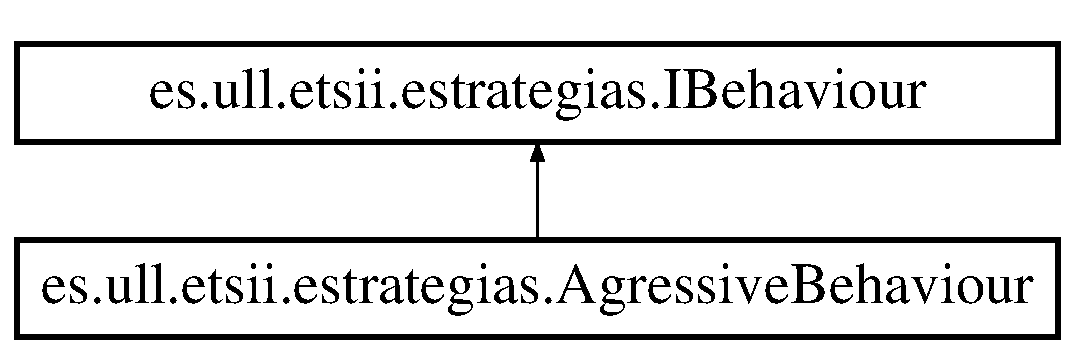
\includegraphics[height=2.000000cm]{classes_1_1ull_1_1etsii_1_1estrategias_1_1_agressive_behaviour}
\end{center}
\end{figure}
\subsection*{Public Member Functions}
\begin{DoxyCompactItemize}
\item 
\hyperlink{classes_1_1ull_1_1etsii_1_1estrategias_1_1_agressive_behaviour_a2925aeed45e4777c845430504878b31c}{Agressive\-Behaviour} ()
\item 
void \hyperlink{classes_1_1ull_1_1etsii_1_1estrategias_1_1_agressive_behaviour_ad7aa2126933c4cb9af2d1341fc21bda5}{move\-Command} ()
\end{DoxyCompactItemize}


\subsection{Detailed Description}
Comportamiento Agresivo. \begin{DoxyAuthor}{Author}
Mauri 
\end{DoxyAuthor}


\subsection{Constructor \& Destructor Documentation}
\hypertarget{classes_1_1ull_1_1etsii_1_1estrategias_1_1_agressive_behaviour_a2925aeed45e4777c845430504878b31c}{\index{es\-::ull\-::etsii\-::estrategias\-::\-Agressive\-Behaviour@{es\-::ull\-::etsii\-::estrategias\-::\-Agressive\-Behaviour}!Agressive\-Behaviour@{Agressive\-Behaviour}}
\index{Agressive\-Behaviour@{Agressive\-Behaviour}!es::ull::etsii::estrategias::AgressiveBehaviour@{es\-::ull\-::etsii\-::estrategias\-::\-Agressive\-Behaviour}}
\subsubsection[{Agressive\-Behaviour}]{\setlength{\rightskip}{0pt plus 5cm}es.\-ull.\-etsii.\-estrategias.\-Agressive\-Behaviour.\-Agressive\-Behaviour (
\begin{DoxyParamCaption}
{}
\end{DoxyParamCaption}
)}}\label{classes_1_1ull_1_1etsii_1_1estrategias_1_1_agressive_behaviour_a2925aeed45e4777c845430504878b31c}


\subsection{Member Function Documentation}
\hypertarget{classes_1_1ull_1_1etsii_1_1estrategias_1_1_agressive_behaviour_ad7aa2126933c4cb9af2d1341fc21bda5}{\index{es\-::ull\-::etsii\-::estrategias\-::\-Agressive\-Behaviour@{es\-::ull\-::etsii\-::estrategias\-::\-Agressive\-Behaviour}!move\-Command@{move\-Command}}
\index{move\-Command@{move\-Command}!es::ull::etsii::estrategias::AgressiveBehaviour@{es\-::ull\-::etsii\-::estrategias\-::\-Agressive\-Behaviour}}
\subsubsection[{move\-Command}]{\setlength{\rightskip}{0pt plus 5cm}void es.\-ull.\-etsii.\-estrategias.\-Agressive\-Behaviour.\-move\-Command (
\begin{DoxyParamCaption}
{}
\end{DoxyParamCaption}
)}}\label{classes_1_1ull_1_1etsii_1_1estrategias_1_1_agressive_behaviour_ad7aa2126933c4cb9af2d1341fc21bda5}
Sobrecarga del comportamiento 

Implements \hyperlink{interfacees_1_1ull_1_1etsii_1_1estrategias_1_1_i_behaviour_a571cbea7f7404a92a599baca57b209b4}{es.\-ull.\-etsii.\-estrategias.\-I\-Behaviour}.



The documentation for this class was generated from the following file\-:\begin{DoxyCompactItemize}
\item 
src/es/ull/etsii/estrategias/\hyperlink{_agressive_behaviour_8java}{Agressive\-Behaviour.\-java}\end{DoxyCompactItemize}

\hypertarget{classes_1_1ull_1_1etsii_1_1estrategias_1_1_defensive_behaviour}{\section{es.\-ull.\-etsii.\-estrategias.\-Defensive\-Behaviour Class Reference}
\label{classes_1_1ull_1_1etsii_1_1estrategias_1_1_defensive_behaviour}\index{es.\-ull.\-etsii.\-estrategias.\-Defensive\-Behaviour@{es.\-ull.\-etsii.\-estrategias.\-Defensive\-Behaviour}}
}
Inheritance diagram for es.\-ull.\-etsii.\-estrategias.\-Defensive\-Behaviour\-:\begin{figure}[H]
\begin{center}
\leavevmode
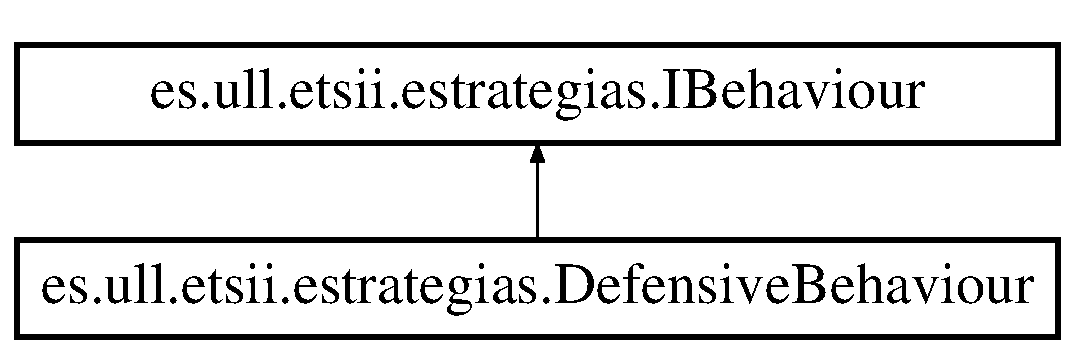
\includegraphics[height=2.000000cm]{classes_1_1ull_1_1etsii_1_1estrategias_1_1_defensive_behaviour}
\end{center}
\end{figure}
\subsection*{Public Member Functions}
\begin{DoxyCompactItemize}
\item 
\hyperlink{classes_1_1ull_1_1etsii_1_1estrategias_1_1_defensive_behaviour_a0c911bd979f9747bfc8e32811f83d122}{Defensive\-Behaviour} ()
\item 
void \hyperlink{classes_1_1ull_1_1etsii_1_1estrategias_1_1_defensive_behaviour_ae42e80d346434436ca75b53b6f2b5e4c}{move\-Command} ()
\end{DoxyCompactItemize}


\subsection{Detailed Description}
Comportamiento defensivo \begin{DoxyAuthor}{Author}
Mauri 
\end{DoxyAuthor}


\subsection{Constructor \& Destructor Documentation}
\hypertarget{classes_1_1ull_1_1etsii_1_1estrategias_1_1_defensive_behaviour_a0c911bd979f9747bfc8e32811f83d122}{\index{es\-::ull\-::etsii\-::estrategias\-::\-Defensive\-Behaviour@{es\-::ull\-::etsii\-::estrategias\-::\-Defensive\-Behaviour}!Defensive\-Behaviour@{Defensive\-Behaviour}}
\index{Defensive\-Behaviour@{Defensive\-Behaviour}!es::ull::etsii::estrategias::DefensiveBehaviour@{es\-::ull\-::etsii\-::estrategias\-::\-Defensive\-Behaviour}}
\subsubsection[{Defensive\-Behaviour}]{\setlength{\rightskip}{0pt plus 5cm}es.\-ull.\-etsii.\-estrategias.\-Defensive\-Behaviour.\-Defensive\-Behaviour (
\begin{DoxyParamCaption}
{}
\end{DoxyParamCaption}
)}}\label{classes_1_1ull_1_1etsii_1_1estrategias_1_1_defensive_behaviour_a0c911bd979f9747bfc8e32811f83d122}


\subsection{Member Function Documentation}
\hypertarget{classes_1_1ull_1_1etsii_1_1estrategias_1_1_defensive_behaviour_ae42e80d346434436ca75b53b6f2b5e4c}{\index{es\-::ull\-::etsii\-::estrategias\-::\-Defensive\-Behaviour@{es\-::ull\-::etsii\-::estrategias\-::\-Defensive\-Behaviour}!move\-Command@{move\-Command}}
\index{move\-Command@{move\-Command}!es::ull::etsii::estrategias::DefensiveBehaviour@{es\-::ull\-::etsii\-::estrategias\-::\-Defensive\-Behaviour}}
\subsubsection[{move\-Command}]{\setlength{\rightskip}{0pt plus 5cm}void es.\-ull.\-etsii.\-estrategias.\-Defensive\-Behaviour.\-move\-Command (
\begin{DoxyParamCaption}
{}
\end{DoxyParamCaption}
)}}\label{classes_1_1ull_1_1etsii_1_1estrategias_1_1_defensive_behaviour_ae42e80d346434436ca75b53b6f2b5e4c}
Sobrecarga del comportamiento 

Implements \hyperlink{interfacees_1_1ull_1_1etsii_1_1estrategias_1_1_i_behaviour_a571cbea7f7404a92a599baca57b209b4}{es.\-ull.\-etsii.\-estrategias.\-I\-Behaviour}.



The documentation for this class was generated from the following file\-:\begin{DoxyCompactItemize}
\item 
src/es/ull/etsii/estrategias/\hyperlink{_defensive_behaviour_8java}{Defensive\-Behaviour.\-java}\end{DoxyCompactItemize}

\hypertarget{interfacees_1_1ull_1_1etsii_1_1estrategias_1_1_i_behaviour}{\section{es.\-ull.\-etsii.\-estrategias.\-I\-Behaviour Interface Reference}
\label{interfacees_1_1ull_1_1etsii_1_1estrategias_1_1_i_behaviour}\index{es.\-ull.\-etsii.\-estrategias.\-I\-Behaviour@{es.\-ull.\-etsii.\-estrategias.\-I\-Behaviour}}
}
Inheritance diagram for es.\-ull.\-etsii.\-estrategias.\-I\-Behaviour\-:\begin{figure}[H]
\begin{center}
\leavevmode
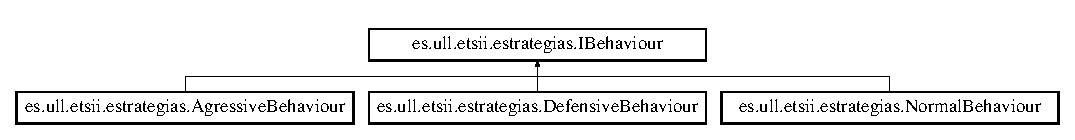
\includegraphics[height=1.435897cm]{interfacees_1_1ull_1_1etsii_1_1estrategias_1_1_i_behaviour}
\end{center}
\end{figure}
\subsection*{Public Member Functions}
\begin{DoxyCompactItemize}
\item 
void \hyperlink{interfacees_1_1ull_1_1etsii_1_1estrategias_1_1_i_behaviour_a571cbea7f7404a92a599baca57b209b4}{move\-Command} ()
\end{DoxyCompactItemize}


\subsection{Detailed Description}
Interfaz de comportamiento \begin{DoxyAuthor}{Author}
Mauri 
\end{DoxyAuthor}


\subsection{Member Function Documentation}
\hypertarget{interfacees_1_1ull_1_1etsii_1_1estrategias_1_1_i_behaviour_a571cbea7f7404a92a599baca57b209b4}{\index{es\-::ull\-::etsii\-::estrategias\-::\-I\-Behaviour@{es\-::ull\-::etsii\-::estrategias\-::\-I\-Behaviour}!move\-Command@{move\-Command}}
\index{move\-Command@{move\-Command}!es::ull::etsii::estrategias::IBehaviour@{es\-::ull\-::etsii\-::estrategias\-::\-I\-Behaviour}}
\subsubsection[{move\-Command}]{\setlength{\rightskip}{0pt plus 5cm}void es.\-ull.\-etsii.\-estrategias.\-I\-Behaviour.\-move\-Command (
\begin{DoxyParamCaption}
{}
\end{DoxyParamCaption}
)}}\label{interfacees_1_1ull_1_1etsii_1_1estrategias_1_1_i_behaviour_a571cbea7f7404a92a599baca57b209b4}


Implemented in \hyperlink{classes_1_1ull_1_1etsii_1_1estrategias_1_1_agressive_behaviour_ad7aa2126933c4cb9af2d1341fc21bda5}{es.\-ull.\-etsii.\-estrategias.\-Agressive\-Behaviour}, \hyperlink{classes_1_1ull_1_1etsii_1_1estrategias_1_1_defensive_behaviour_ae42e80d346434436ca75b53b6f2b5e4c}{es.\-ull.\-etsii.\-estrategias.\-Defensive\-Behaviour}, and \hyperlink{classes_1_1ull_1_1etsii_1_1estrategias_1_1_normal_behaviour_a746dcf0cdc749b5b836e2c1bcbb4e7ee}{es.\-ull.\-etsii.\-estrategias.\-Normal\-Behaviour}.



The documentation for this interface was generated from the following file\-:\begin{DoxyCompactItemize}
\item 
src/es/ull/etsii/estrategias/\hyperlink{_i_behaviour_8java}{I\-Behaviour.\-java}\end{DoxyCompactItemize}

\hypertarget{classes_1_1ull_1_1etsii_1_1main_1_1_main}{\section{es.\-ull.\-etsii.\-main.\-Main Class Reference}
\label{classes_1_1ull_1_1etsii_1_1main_1_1_main}\index{es.\-ull.\-etsii.\-main.\-Main@{es.\-ull.\-etsii.\-main.\-Main}}
}
\subsection*{Static Public Member Functions}
\begin{DoxyCompactItemize}
\item 
static void \hyperlink{classes_1_1ull_1_1etsii_1_1main_1_1_main_adb143ab65570fbdbe17f7c1ab58c71bd}{main} (String\mbox{[}$\,$\mbox{]} args)
\end{DoxyCompactItemize}


\subsection{Detailed Description}
Clase principal \begin{DoxyAuthor}{Author}
Mauri 
\end{DoxyAuthor}


\subsection{Member Function Documentation}
\hypertarget{classes_1_1ull_1_1etsii_1_1main_1_1_main_adb143ab65570fbdbe17f7c1ab58c71bd}{\index{es\-::ull\-::etsii\-::main\-::\-Main@{es\-::ull\-::etsii\-::main\-::\-Main}!main@{main}}
\index{main@{main}!es::ull::etsii::main::Main@{es\-::ull\-::etsii\-::main\-::\-Main}}
\subsubsection[{main}]{\setlength{\rightskip}{0pt plus 5cm}static void es.\-ull.\-etsii.\-main.\-Main.\-main (
\begin{DoxyParamCaption}
\item[{String\mbox{[}$\,$\mbox{]}}]{args}
\end{DoxyParamCaption}
)\hspace{0.3cm}{\ttfamily [static]}}}\label{classes_1_1ull_1_1etsii_1_1main_1_1_main_adb143ab65570fbdbe17f7c1ab58c71bd}


The documentation for this class was generated from the following file\-:\begin{DoxyCompactItemize}
\item 
src/es/ull/etsii/main/\hyperlink{_main_8java}{Main.\-java}\end{DoxyCompactItemize}

\hypertarget{classes_1_1ull_1_1etsii_1_1estrategias_1_1_normal_behaviour}{\section{es.\-ull.\-etsii.\-estrategias.\-Normal\-Behaviour Class Reference}
\label{classes_1_1ull_1_1etsii_1_1estrategias_1_1_normal_behaviour}\index{es.\-ull.\-etsii.\-estrategias.\-Normal\-Behaviour@{es.\-ull.\-etsii.\-estrategias.\-Normal\-Behaviour}}
}
Inheritance diagram for es.\-ull.\-etsii.\-estrategias.\-Normal\-Behaviour\-:\begin{figure}[H]
\begin{center}
\leavevmode
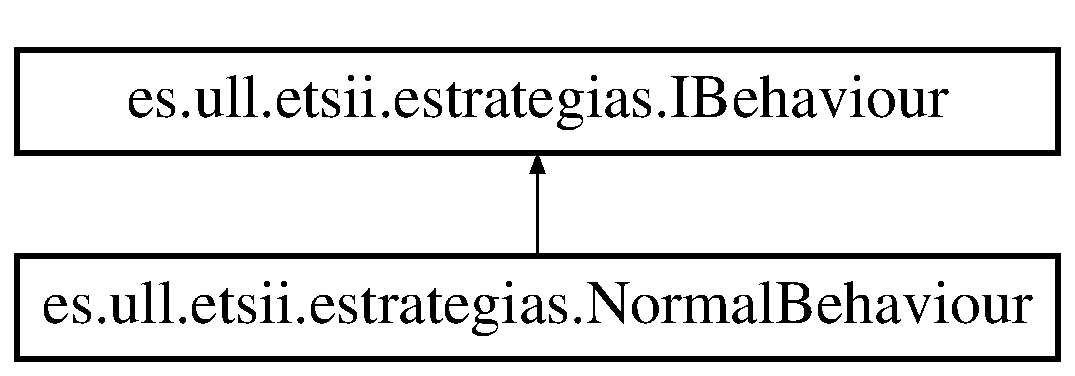
\includegraphics[height=2.000000cm]{classes_1_1ull_1_1etsii_1_1estrategias_1_1_normal_behaviour}
\end{center}
\end{figure}
\subsection*{Public Member Functions}
\begin{DoxyCompactItemize}
\item 
\hyperlink{classes_1_1ull_1_1etsii_1_1estrategias_1_1_normal_behaviour_ab63f550e80f2f3a3de147511b7cd8cff}{Normal\-Behaviour} ()
\item 
void \hyperlink{classes_1_1ull_1_1etsii_1_1estrategias_1_1_normal_behaviour_a746dcf0cdc749b5b836e2c1bcbb4e7ee}{move\-Command} ()
\end{DoxyCompactItemize}


\subsection{Detailed Description}
Comportamiento Normal \begin{DoxyAuthor}{Author}
Mauri 
\end{DoxyAuthor}


\subsection{Constructor \& Destructor Documentation}
\hypertarget{classes_1_1ull_1_1etsii_1_1estrategias_1_1_normal_behaviour_ab63f550e80f2f3a3de147511b7cd8cff}{\index{es\-::ull\-::etsii\-::estrategias\-::\-Normal\-Behaviour@{es\-::ull\-::etsii\-::estrategias\-::\-Normal\-Behaviour}!Normal\-Behaviour@{Normal\-Behaviour}}
\index{Normal\-Behaviour@{Normal\-Behaviour}!es::ull::etsii::estrategias::NormalBehaviour@{es\-::ull\-::etsii\-::estrategias\-::\-Normal\-Behaviour}}
\subsubsection[{Normal\-Behaviour}]{\setlength{\rightskip}{0pt plus 5cm}es.\-ull.\-etsii.\-estrategias.\-Normal\-Behaviour.\-Normal\-Behaviour (
\begin{DoxyParamCaption}
{}
\end{DoxyParamCaption}
)}}\label{classes_1_1ull_1_1etsii_1_1estrategias_1_1_normal_behaviour_ab63f550e80f2f3a3de147511b7cd8cff}


\subsection{Member Function Documentation}
\hypertarget{classes_1_1ull_1_1etsii_1_1estrategias_1_1_normal_behaviour_a746dcf0cdc749b5b836e2c1bcbb4e7ee}{\index{es\-::ull\-::etsii\-::estrategias\-::\-Normal\-Behaviour@{es\-::ull\-::etsii\-::estrategias\-::\-Normal\-Behaviour}!move\-Command@{move\-Command}}
\index{move\-Command@{move\-Command}!es::ull::etsii::estrategias::NormalBehaviour@{es\-::ull\-::etsii\-::estrategias\-::\-Normal\-Behaviour}}
\subsubsection[{move\-Command}]{\setlength{\rightskip}{0pt plus 5cm}void es.\-ull.\-etsii.\-estrategias.\-Normal\-Behaviour.\-move\-Command (
\begin{DoxyParamCaption}
{}
\end{DoxyParamCaption}
)}}\label{classes_1_1ull_1_1etsii_1_1estrategias_1_1_normal_behaviour_a746dcf0cdc749b5b836e2c1bcbb4e7ee}
Sobrecarga del comportamiento 

Implements \hyperlink{interfacees_1_1ull_1_1etsii_1_1estrategias_1_1_i_behaviour_a571cbea7f7404a92a599baca57b209b4}{es.\-ull.\-etsii.\-estrategias.\-I\-Behaviour}.



The documentation for this class was generated from the following file\-:\begin{DoxyCompactItemize}
\item 
src/es/ull/etsii/estrategias/\hyperlink{_normal_behaviour_8java}{Normal\-Behaviour.\-java}\end{DoxyCompactItemize}

\hypertarget{classes_1_1ull_1_1etsii_1_1contexto_1_1_robot}{\section{es.\-ull.\-etsii.\-contexto.\-Robot Class Reference}
\label{classes_1_1ull_1_1etsii_1_1contexto_1_1_robot}\index{es.\-ull.\-etsii.\-contexto.\-Robot@{es.\-ull.\-etsii.\-contexto.\-Robot}}
}
\subsection*{Public Member Functions}
\begin{DoxyCompactItemize}
\item 
\hyperlink{classes_1_1ull_1_1etsii_1_1contexto_1_1_robot_a0d7b2089d4e09dd35a6f5c18a2b5297f}{Robot} ()
\item 
\hyperlink{classes_1_1ull_1_1etsii_1_1contexto_1_1_robot_a2ef4413c2c395c55ad9511aab22c27b5}{Robot} (\hyperlink{interfacees_1_1ull_1_1etsii_1_1estrategias_1_1_i_behaviour}{I\-Behaviour} b)
\item 
void \hyperlink{classes_1_1ull_1_1etsii_1_1contexto_1_1_robot_aaec45e06f689fec583cf168ed28f2d59}{move} ()
\end{DoxyCompactItemize}
\subsection*{Private Attributes}
\begin{DoxyCompactItemize}
\item 
\hyperlink{interfacees_1_1ull_1_1etsii_1_1estrategias_1_1_i_behaviour}{I\-Behaviour} \hyperlink{classes_1_1ull_1_1etsii_1_1contexto_1_1_robot_aebafde0ad8d25d829a8ce4f8287c262f}{strategy}
\end{DoxyCompactItemize}


\subsection{Detailed Description}
Clase que cambia su comportamiento. \begin{DoxyAuthor}{Author}
Mauri 
\end{DoxyAuthor}


\subsection{Constructor \& Destructor Documentation}
\hypertarget{classes_1_1ull_1_1etsii_1_1contexto_1_1_robot_a0d7b2089d4e09dd35a6f5c18a2b5297f}{\index{es\-::ull\-::etsii\-::contexto\-::\-Robot@{es\-::ull\-::etsii\-::contexto\-::\-Robot}!Robot@{Robot}}
\index{Robot@{Robot}!es::ull::etsii::contexto::Robot@{es\-::ull\-::etsii\-::contexto\-::\-Robot}}
\subsubsection[{Robot}]{\setlength{\rightskip}{0pt plus 5cm}es.\-ull.\-etsii.\-contexto.\-Robot.\-Robot (
\begin{DoxyParamCaption}
{}
\end{DoxyParamCaption}
)}}\label{classes_1_1ull_1_1etsii_1_1contexto_1_1_robot_a0d7b2089d4e09dd35a6f5c18a2b5297f}
\hypertarget{classes_1_1ull_1_1etsii_1_1contexto_1_1_robot_a2ef4413c2c395c55ad9511aab22c27b5}{\index{es\-::ull\-::etsii\-::contexto\-::\-Robot@{es\-::ull\-::etsii\-::contexto\-::\-Robot}!Robot@{Robot}}
\index{Robot@{Robot}!es::ull::etsii::contexto::Robot@{es\-::ull\-::etsii\-::contexto\-::\-Robot}}
\subsubsection[{Robot}]{\setlength{\rightskip}{0pt plus 5cm}es.\-ull.\-etsii.\-contexto.\-Robot.\-Robot (
\begin{DoxyParamCaption}
\item[{{\bf I\-Behaviour}}]{b}
\end{DoxyParamCaption}
)}}\label{classes_1_1ull_1_1etsii_1_1contexto_1_1_robot_a2ef4413c2c395c55ad9511aab22c27b5}


\subsection{Member Function Documentation}
\hypertarget{classes_1_1ull_1_1etsii_1_1contexto_1_1_robot_aaec45e06f689fec583cf168ed28f2d59}{\index{es\-::ull\-::etsii\-::contexto\-::\-Robot@{es\-::ull\-::etsii\-::contexto\-::\-Robot}!move@{move}}
\index{move@{move}!es::ull::etsii::contexto::Robot@{es\-::ull\-::etsii\-::contexto\-::\-Robot}}
\subsubsection[{move}]{\setlength{\rightskip}{0pt plus 5cm}void es.\-ull.\-etsii.\-contexto.\-Robot.\-move (
\begin{DoxyParamCaption}
{}
\end{DoxyParamCaption}
)}}\label{classes_1_1ull_1_1etsii_1_1contexto_1_1_robot_aaec45e06f689fec583cf168ed28f2d59}


\subsection{Member Data Documentation}
\hypertarget{classes_1_1ull_1_1etsii_1_1contexto_1_1_robot_aebafde0ad8d25d829a8ce4f8287c262f}{\index{es\-::ull\-::etsii\-::contexto\-::\-Robot@{es\-::ull\-::etsii\-::contexto\-::\-Robot}!strategy@{strategy}}
\index{strategy@{strategy}!es::ull::etsii::contexto::Robot@{es\-::ull\-::etsii\-::contexto\-::\-Robot}}
\subsubsection[{strategy}]{\setlength{\rightskip}{0pt plus 5cm}{\bf I\-Behaviour} es.\-ull.\-etsii.\-contexto.\-Robot.\-strategy\hspace{0.3cm}{\ttfamily [private]}}}\label{classes_1_1ull_1_1etsii_1_1contexto_1_1_robot_aebafde0ad8d25d829a8ce4f8287c262f}


The documentation for this class was generated from the following file\-:\begin{DoxyCompactItemize}
\item 
src/es/ull/etsii/contexto/\hyperlink{_robot_8java}{Robot.\-java}\end{DoxyCompactItemize}

\hypertarget{classes_1_1ull_1_1etsii_1_1singleton_1_1_world}{\section{es.\-ull.\-etsii.\-singleton.\-World Class Reference}
\label{classes_1_1ull_1_1etsii_1_1singleton_1_1_world}\index{es.\-ull.\-etsii.\-singleton.\-World@{es.\-ull.\-etsii.\-singleton.\-World}}
}
\subsection*{Public Member Functions}
\begin{DoxyCompactItemize}
\item 
void \hyperlink{classes_1_1ull_1_1etsii_1_1singleton_1_1_world_af5283e442493b5883cd29f1409632ccb}{play} ()
\item 
Array\-List$<$ \hyperlink{classes_1_1ull_1_1etsii_1_1contexto_1_1_robot}{Robot} $>$ \hyperlink{classes_1_1ull_1_1etsii_1_1singleton_1_1_world_a72ec11603e44fd39d81ca7100eb5b099}{get\-Enjambre} ()
\item 
String \hyperlink{classes_1_1ull_1_1etsii_1_1singleton_1_1_world_a8ad3afa3bcfd8f64134cab1a614e65e0}{get\-Robot\-Reina} ()
\item 
void \hyperlink{classes_1_1ull_1_1etsii_1_1singleton_1_1_world_a99fbb2fc4c1d74fcfb46c3e1d41e6a00}{set\-Robot\-Reina} (String \hyperlink{classes_1_1ull_1_1etsii_1_1singleton_1_1_world_a1f5f27f29afee7ed72993e7c135eadea}{robot\-Reina})
\end{DoxyCompactItemize}
\subsection*{Static Public Member Functions}
\begin{DoxyCompactItemize}
\item 
static \hyperlink{classes_1_1ull_1_1etsii_1_1singleton_1_1_world}{World} \hyperlink{classes_1_1ull_1_1etsii_1_1singleton_1_1_world_a19de9b4dd733fd5dbd2e3d32f9c874f0}{get\-World} ()
\end{DoxyCompactItemize}
\subsection*{Protected Attributes}
\begin{DoxyCompactItemize}
\item 
Array\-List$<$ \hyperlink{classes_1_1ull_1_1etsii_1_1contexto_1_1_robot}{Robot} $>$ \hyperlink{classes_1_1ull_1_1etsii_1_1singleton_1_1_world_ac734bf40937588aa531202789f1e694d}{enjambre}
\item 
String \hyperlink{classes_1_1ull_1_1etsii_1_1singleton_1_1_world_a1f5f27f29afee7ed72993e7c135eadea}{robot\-Reina}
\end{DoxyCompactItemize}
\subsection*{Private Member Functions}
\begin{DoxyCompactItemize}
\item 
\hyperlink{classes_1_1ull_1_1etsii_1_1singleton_1_1_world_a93a6260b037ea9be5a05e2d48d671ca4}{World} ()
\item 
int \hyperlink{classes_1_1ull_1_1etsii_1_1singleton_1_1_world_a7a9a245c4e14a434d3198ac54776c9ea}{num\-Aleatorio} ()
\end{DoxyCompactItemize}
\subsection*{Static Private Attributes}
\begin{DoxyCompactItemize}
\item 
static \hyperlink{classes_1_1ull_1_1etsii_1_1singleton_1_1_world}{World} \hyperlink{classes_1_1ull_1_1etsii_1_1singleton_1_1_world_af1f0c7ac3c0f00f44d582ada43659948}{instance} = new \hyperlink{classes_1_1ull_1_1etsii_1_1singleton_1_1_world}{World}()
\end{DoxyCompactItemize}


\subsection{Detailed Description}
Clase que utiliza el patr�n singleton para controlar un enjambre de robots desde diferentes planetas. \begin{DoxyAuthor}{Author}
Mauri 
\end{DoxyAuthor}


\subsection{Constructor \& Destructor Documentation}
\hypertarget{classes_1_1ull_1_1etsii_1_1singleton_1_1_world_a93a6260b037ea9be5a05e2d48d671ca4}{\index{es\-::ull\-::etsii\-::singleton\-::\-World@{es\-::ull\-::etsii\-::singleton\-::\-World}!World@{World}}
\index{World@{World}!es::ull::etsii::singleton::World@{es\-::ull\-::etsii\-::singleton\-::\-World}}
\subsubsection[{World}]{\setlength{\rightskip}{0pt plus 5cm}es.\-ull.\-etsii.\-singleton.\-World.\-World (
\begin{DoxyParamCaption}
{}
\end{DoxyParamCaption}
)\hspace{0.3cm}{\ttfamily [private]}}}\label{classes_1_1ull_1_1etsii_1_1singleton_1_1_world_a93a6260b037ea9be5a05e2d48d671ca4}


\subsection{Member Function Documentation}
\hypertarget{classes_1_1ull_1_1etsii_1_1singleton_1_1_world_a72ec11603e44fd39d81ca7100eb5b099}{\index{es\-::ull\-::etsii\-::singleton\-::\-World@{es\-::ull\-::etsii\-::singleton\-::\-World}!get\-Enjambre@{get\-Enjambre}}
\index{get\-Enjambre@{get\-Enjambre}!es::ull::etsii::singleton::World@{es\-::ull\-::etsii\-::singleton\-::\-World}}
\subsubsection[{get\-Enjambre}]{\setlength{\rightskip}{0pt plus 5cm}Array\-List$<${\bf Robot}$>$ es.\-ull.\-etsii.\-singleton.\-World.\-get\-Enjambre (
\begin{DoxyParamCaption}
{}
\end{DoxyParamCaption}
)}}\label{classes_1_1ull_1_1etsii_1_1singleton_1_1_world_a72ec11603e44fd39d81ca7100eb5b099}
Acceso al enjambre de robots \begin{DoxyReturn}{Returns}
devuelve un array de robots 
\end{DoxyReturn}
\hypertarget{classes_1_1ull_1_1etsii_1_1singleton_1_1_world_a8ad3afa3bcfd8f64134cab1a614e65e0}{\index{es\-::ull\-::etsii\-::singleton\-::\-World@{es\-::ull\-::etsii\-::singleton\-::\-World}!get\-Robot\-Reina@{get\-Robot\-Reina}}
\index{get\-Robot\-Reina@{get\-Robot\-Reina}!es::ull::etsii::singleton::World@{es\-::ull\-::etsii\-::singleton\-::\-World}}
\subsubsection[{get\-Robot\-Reina}]{\setlength{\rightskip}{0pt plus 5cm}String es.\-ull.\-etsii.\-singleton.\-World.\-get\-Robot\-Reina (
\begin{DoxyParamCaption}
{}
\end{DoxyParamCaption}
)}}\label{classes_1_1ull_1_1etsii_1_1singleton_1_1_world_a8ad3afa3bcfd8f64134cab1a614e65e0}
\hypertarget{classes_1_1ull_1_1etsii_1_1singleton_1_1_world_a19de9b4dd733fd5dbd2e3d32f9c874f0}{\index{es\-::ull\-::etsii\-::singleton\-::\-World@{es\-::ull\-::etsii\-::singleton\-::\-World}!get\-World@{get\-World}}
\index{get\-World@{get\-World}!es::ull::etsii::singleton::World@{es\-::ull\-::etsii\-::singleton\-::\-World}}
\subsubsection[{get\-World}]{\setlength{\rightskip}{0pt plus 5cm}static {\bf World} es.\-ull.\-etsii.\-singleton.\-World.\-get\-World (
\begin{DoxyParamCaption}
{}
\end{DoxyParamCaption}
)\hspace{0.3cm}{\ttfamily [static]}}}\label{classes_1_1ull_1_1etsii_1_1singleton_1_1_world_a19de9b4dd733fd5dbd2e3d32f9c874f0}
Metodo de creacion de instancia unica \begin{DoxyReturn}{Returns}
la instancia del metodo singleton 
\end{DoxyReturn}
\hypertarget{classes_1_1ull_1_1etsii_1_1singleton_1_1_world_a7a9a245c4e14a434d3198ac54776c9ea}{\index{es\-::ull\-::etsii\-::singleton\-::\-World@{es\-::ull\-::etsii\-::singleton\-::\-World}!num\-Aleatorio@{num\-Aleatorio}}
\index{num\-Aleatorio@{num\-Aleatorio}!es::ull::etsii::singleton::World@{es\-::ull\-::etsii\-::singleton\-::\-World}}
\subsubsection[{num\-Aleatorio}]{\setlength{\rightskip}{0pt plus 5cm}int es.\-ull.\-etsii.\-singleton.\-World.\-num\-Aleatorio (
\begin{DoxyParamCaption}
{}
\end{DoxyParamCaption}
)\hspace{0.3cm}{\ttfamily [private]}}}\label{classes_1_1ull_1_1etsii_1_1singleton_1_1_world_a7a9a245c4e14a434d3198ac54776c9ea}
Calcula un numero aleatorio \begin{DoxyReturn}{Returns}
nuemro entre 0 y 2 
\end{DoxyReturn}
\hypertarget{classes_1_1ull_1_1etsii_1_1singleton_1_1_world_af5283e442493b5883cd29f1409632ccb}{\index{es\-::ull\-::etsii\-::singleton\-::\-World@{es\-::ull\-::etsii\-::singleton\-::\-World}!play@{play}}
\index{play@{play}!es::ull::etsii::singleton::World@{es\-::ull\-::etsii\-::singleton\-::\-World}}
\subsubsection[{play}]{\setlength{\rightskip}{0pt plus 5cm}void es.\-ull.\-etsii.\-singleton.\-World.\-play (
\begin{DoxyParamCaption}
{}
\end{DoxyParamCaption}
)}}\label{classes_1_1ull_1_1etsii_1_1singleton_1_1_world_af5283e442493b5883cd29f1409632ccb}
Cambia el estado de los robot que forman el enjambre \hypertarget{classes_1_1ull_1_1etsii_1_1singleton_1_1_world_a99fbb2fc4c1d74fcfb46c3e1d41e6a00}{\index{es\-::ull\-::etsii\-::singleton\-::\-World@{es\-::ull\-::etsii\-::singleton\-::\-World}!set\-Robot\-Reina@{set\-Robot\-Reina}}
\index{set\-Robot\-Reina@{set\-Robot\-Reina}!es::ull::etsii::singleton::World@{es\-::ull\-::etsii\-::singleton\-::\-World}}
\subsubsection[{set\-Robot\-Reina}]{\setlength{\rightskip}{0pt plus 5cm}void es.\-ull.\-etsii.\-singleton.\-World.\-set\-Robot\-Reina (
\begin{DoxyParamCaption}
\item[{String}]{robot\-Reina}
\end{DoxyParamCaption}
)}}\label{classes_1_1ull_1_1etsii_1_1singleton_1_1_world_a99fbb2fc4c1d74fcfb46c3e1d41e6a00}


\subsection{Member Data Documentation}
\hypertarget{classes_1_1ull_1_1etsii_1_1singleton_1_1_world_ac734bf40937588aa531202789f1e694d}{\index{es\-::ull\-::etsii\-::singleton\-::\-World@{es\-::ull\-::etsii\-::singleton\-::\-World}!enjambre@{enjambre}}
\index{enjambre@{enjambre}!es::ull::etsii::singleton::World@{es\-::ull\-::etsii\-::singleton\-::\-World}}
\subsubsection[{enjambre}]{\setlength{\rightskip}{0pt plus 5cm}Array\-List$<${\bf Robot}$>$ es.\-ull.\-etsii.\-singleton.\-World.\-enjambre\hspace{0.3cm}{\ttfamily [protected]}}}\label{classes_1_1ull_1_1etsii_1_1singleton_1_1_world_ac734bf40937588aa531202789f1e694d}
\hypertarget{classes_1_1ull_1_1etsii_1_1singleton_1_1_world_af1f0c7ac3c0f00f44d582ada43659948}{\index{es\-::ull\-::etsii\-::singleton\-::\-World@{es\-::ull\-::etsii\-::singleton\-::\-World}!instance@{instance}}
\index{instance@{instance}!es::ull::etsii::singleton::World@{es\-::ull\-::etsii\-::singleton\-::\-World}}
\subsubsection[{instance}]{\setlength{\rightskip}{0pt plus 5cm}{\bf World} es.\-ull.\-etsii.\-singleton.\-World.\-instance = new {\bf World}()\hspace{0.3cm}{\ttfamily [static]}, {\ttfamily [private]}}}\label{classes_1_1ull_1_1etsii_1_1singleton_1_1_world_af1f0c7ac3c0f00f44d582ada43659948}
\hypertarget{classes_1_1ull_1_1etsii_1_1singleton_1_1_world_a1f5f27f29afee7ed72993e7c135eadea}{\index{es\-::ull\-::etsii\-::singleton\-::\-World@{es\-::ull\-::etsii\-::singleton\-::\-World}!robot\-Reina@{robot\-Reina}}
\index{robot\-Reina@{robot\-Reina}!es::ull::etsii::singleton::World@{es\-::ull\-::etsii\-::singleton\-::\-World}}
\subsubsection[{robot\-Reina}]{\setlength{\rightskip}{0pt plus 5cm}String es.\-ull.\-etsii.\-singleton.\-World.\-robot\-Reina\hspace{0.3cm}{\ttfamily [protected]}}}\label{classes_1_1ull_1_1etsii_1_1singleton_1_1_world_a1f5f27f29afee7ed72993e7c135eadea}


The documentation for this class was generated from the following file\-:\begin{DoxyCompactItemize}
\item 
src/es/ull/etsii/singleton/\hyperlink{_world_8java}{World.\-java}\end{DoxyCompactItemize}

\chapter{File Documentation}
\hypertarget{_robot_8java}{\section{src/es/ull/etsii/contexto/\-Robot.java File Reference}
\label{_robot_8java}\index{src/es/ull/etsii/contexto/\-Robot.\-java@{src/es/ull/etsii/contexto/\-Robot.\-java}}
}
\subsection*{Classes}
\begin{DoxyCompactItemize}
\item 
class \hyperlink{classes_1_1ull_1_1etsii_1_1contexto_1_1_robot}{es.\-ull.\-etsii.\-contexto.\-Robot}
\end{DoxyCompactItemize}
\subsection*{Packages}
\begin{DoxyCompactItemize}
\item 
package \hyperlink{namespacees_1_1ull_1_1etsii_1_1contexto}{es.\-ull.\-etsii.\-contexto}
\end{DoxyCompactItemize}

\hypertarget{_agressive_behaviour_8java}{\section{src/es/ull/etsii/estrategias/\-Agressive\-Behaviour.java File Reference}
\label{_agressive_behaviour_8java}\index{src/es/ull/etsii/estrategias/\-Agressive\-Behaviour.\-java@{src/es/ull/etsii/estrategias/\-Agressive\-Behaviour.\-java}}
}
\subsection*{Classes}
\begin{DoxyCompactItemize}
\item 
class \hyperlink{classes_1_1ull_1_1etsii_1_1estrategias_1_1_agressive_behaviour}{es.\-ull.\-etsii.\-estrategias.\-Agressive\-Behaviour}
\end{DoxyCompactItemize}
\subsection*{Packages}
\begin{DoxyCompactItemize}
\item 
package \hyperlink{namespacees_1_1ull_1_1etsii_1_1estrategias}{es.\-ull.\-etsii.\-estrategias}
\end{DoxyCompactItemize}

\hypertarget{_defensive_behaviour_8java}{\section{src/es/ull/etsii/estrategias/\-Defensive\-Behaviour.java File Reference}
\label{_defensive_behaviour_8java}\index{src/es/ull/etsii/estrategias/\-Defensive\-Behaviour.\-java@{src/es/ull/etsii/estrategias/\-Defensive\-Behaviour.\-java}}
}
\subsection*{Classes}
\begin{DoxyCompactItemize}
\item 
class \hyperlink{classes_1_1ull_1_1etsii_1_1estrategias_1_1_defensive_behaviour}{es.\-ull.\-etsii.\-estrategias.\-Defensive\-Behaviour}
\end{DoxyCompactItemize}
\subsection*{Packages}
\begin{DoxyCompactItemize}
\item 
package \hyperlink{namespacees_1_1ull_1_1etsii_1_1estrategias}{es.\-ull.\-etsii.\-estrategias}
\end{DoxyCompactItemize}

\hypertarget{_i_behaviour_8java}{\section{src/es/ull/etsii/estrategias/\-I\-Behaviour.java File Reference}
\label{_i_behaviour_8java}\index{src/es/ull/etsii/estrategias/\-I\-Behaviour.\-java@{src/es/ull/etsii/estrategias/\-I\-Behaviour.\-java}}
}
\subsection*{Classes}
\begin{DoxyCompactItemize}
\item 
interface \hyperlink{interfacees_1_1ull_1_1etsii_1_1estrategias_1_1_i_behaviour}{es.\-ull.\-etsii.\-estrategias.\-I\-Behaviour}
\end{DoxyCompactItemize}
\subsection*{Packages}
\begin{DoxyCompactItemize}
\item 
package \hyperlink{namespacees_1_1ull_1_1etsii_1_1estrategias}{es.\-ull.\-etsii.\-estrategias}
\end{DoxyCompactItemize}

\hypertarget{_normal_behaviour_8java}{\section{src/es/ull/etsii/estrategias/\-Normal\-Behaviour.java File Reference}
\label{_normal_behaviour_8java}\index{src/es/ull/etsii/estrategias/\-Normal\-Behaviour.\-java@{src/es/ull/etsii/estrategias/\-Normal\-Behaviour.\-java}}
}
\subsection*{Classes}
\begin{DoxyCompactItemize}
\item 
class \hyperlink{classes_1_1ull_1_1etsii_1_1estrategias_1_1_normal_behaviour}{es.\-ull.\-etsii.\-estrategias.\-Normal\-Behaviour}
\end{DoxyCompactItemize}
\subsection*{Packages}
\begin{DoxyCompactItemize}
\item 
package \hyperlink{namespacees_1_1ull_1_1etsii_1_1estrategias}{es.\-ull.\-etsii.\-estrategias}
\end{DoxyCompactItemize}

\hypertarget{_main_8java}{\section{src/es/ull/etsii/main/\-Main.java File Reference}
\label{_main_8java}\index{src/es/ull/etsii/main/\-Main.\-java@{src/es/ull/etsii/main/\-Main.\-java}}
}
\subsection*{Classes}
\begin{DoxyCompactItemize}
\item 
class \hyperlink{classes_1_1ull_1_1etsii_1_1main_1_1_main}{es.\-ull.\-etsii.\-main.\-Main}
\end{DoxyCompactItemize}
\subsection*{Packages}
\begin{DoxyCompactItemize}
\item 
package \hyperlink{namespacees_1_1ull_1_1etsii_1_1main}{es.\-ull.\-etsii.\-main}
\end{DoxyCompactItemize}

\hypertarget{_world_8java}{\section{src/es/ull/etsii/singleton/\-World.java File Reference}
\label{_world_8java}\index{src/es/ull/etsii/singleton/\-World.\-java@{src/es/ull/etsii/singleton/\-World.\-java}}
}
\subsection*{Classes}
\begin{DoxyCompactItemize}
\item 
class \hyperlink{classes_1_1ull_1_1etsii_1_1singleton_1_1_world}{es.\-ull.\-etsii.\-singleton.\-World}
\end{DoxyCompactItemize}
\subsection*{Packages}
\begin{DoxyCompactItemize}
\item 
package \hyperlink{namespacees_1_1ull_1_1etsii_1_1singleton}{es.\-ull.\-etsii.\-singleton}
\end{DoxyCompactItemize}

%--- End generated contents ---

% Index
\newpage
\phantomsection
\addcontentsline{toc}{part}{Index}
\printindex

\end{document}
